\documentclass[12pt]{article}

%% preamble: Keep it clean; only include those you need
\usepackage{amsmath}
\usepackage[margin = 1in]{geometry}
\usepackage{graphicx}
\usepackage{booktabs}
\usepackage{natbib}

% for space filling
\usepackage{lipsum}
% highlighting hyper links
\usepackage[colorlinks=true, citecolor=blue]{hyperref}


%% meta data

\title{Stats Paper HW 2}
\author{Alexander Rice\\
  Department of Statistics\\
  University of Connecticut
}

\begin{document}
\maketitle

\begin{abstract}
Abstract goes here.  
\end{abstract}


\section{Introduction}
\label{sec:intro}

Use this section to answer three questions:
Why is the topic important/interesting?
What has been done on this topic in the literature?
What is your contribution?

\lipsum[1-3]

To cite a reference, here are examples.
\citet{Kim2019analysis} did something ... \lipsum[1]

A lot of work has been done \citep[e.g.,][]{Kim2019analysis}.
\lipsum[2]
Some parametric bootstrap sample size approach was proposed by
\citet{Villela2019analysis}. 


% roadmap
The rest of the paper is organized as follows.
The data will be presented in Section~\ref{sec:data}.
The methods are described in Section~\ref{sec:meth}.
The results are reported in Section~\ref{sec:resu}.
A discussion concludes in Section~\ref{sec:disc}.


\section{Data}
\label{sec:data}

Use this section to describe the data that helps to answer your research
questions. Recall specific heat capacity
\begin{equation}
  \label{eq:heat}
  q = mc\Delta T
\end{equation}
which models the heat lost in a sample $q$ calculated with $m$ mass, $c$ is specific heat capacity, and $\Delta T$ is the temperature change.
\lipsum{1}

\section{Methods}
\label{sec:meth}

Use this section to present the methodologies that will generate results by
analyzing the data. Suppose that we have a right triangle. We can model the side lengths with the Pythagorean theorem which is
\begin{equation}
  \label{eq:area}
  a^2 + b^2 = c^2
\end{equation}

Equation~\eqref{eq:area} is interesting. \lipsum[1-4]

Sometimes I don't want an equation to be numbered such as this one:
\[
  x = \frac{-b \pm \sqrt{b^2 - 4ac}}{2a},
\]
which is the quadratic formula.



\section{Results}
\label{sec:resu}

Table~\ref{tab:rv} summarizes some example draws from some distributions.
\lipsum[1-4]

\begin{table}[tbp]
  \caption{This is my first table.}
  \label{tab:rv}
\centering
\begin{tabular}{rrr}
  \toprule
trial & meters & seconds \\ 
  \midrule
1 & 16.789 & 2.401 \\ 
  2 & 15.408 & 3.529 \\ 
  3 & 79.230 & 2.112 \\ 
  4 & 69.696 & 11.111 \\ 
  5 & 1.086 & 50.921 \\ 
  6 & 0.001 & 13.012 \\ 
  7 & 50.067 & 120.230 \\ 
  8 & 80.367 & 4.016 \\ 
  9 & 1.111 & 13.404 \\ 
  10 & 4.23 & 12.101 \\ 
   \bottomrule
\end{tabular}
\end{table}

Figure~\ref{fig:USarrests} shows the distance against the speed from this dataset.


\begin{figure}[tbp]
  \centering
  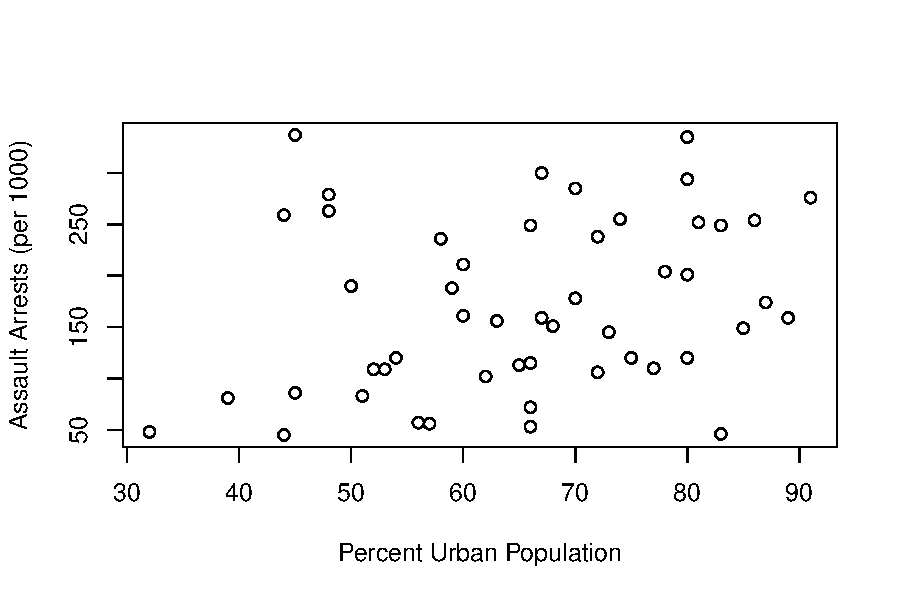
\includegraphics[width=\textwidth]{USarrests.pdf}
  \caption{This is my first figure.}
  \label{fig:USarrests}
\end{figure}

\section{Discussion}
\label{sec:disc}

What are the main contributions again?

What are the limitations of this study?

What are worth pursuing further in the future?

\lipsum[1-2]
Watch for prevalence of diabetes \citep{Tiancai2019analysis}.

\bibliography{refs}
\bibliographystyle{mcap}

\end{document}